\chapter{船岸连接监控与控制系统设计}

\begin{figure}[!htp]
	\centering
	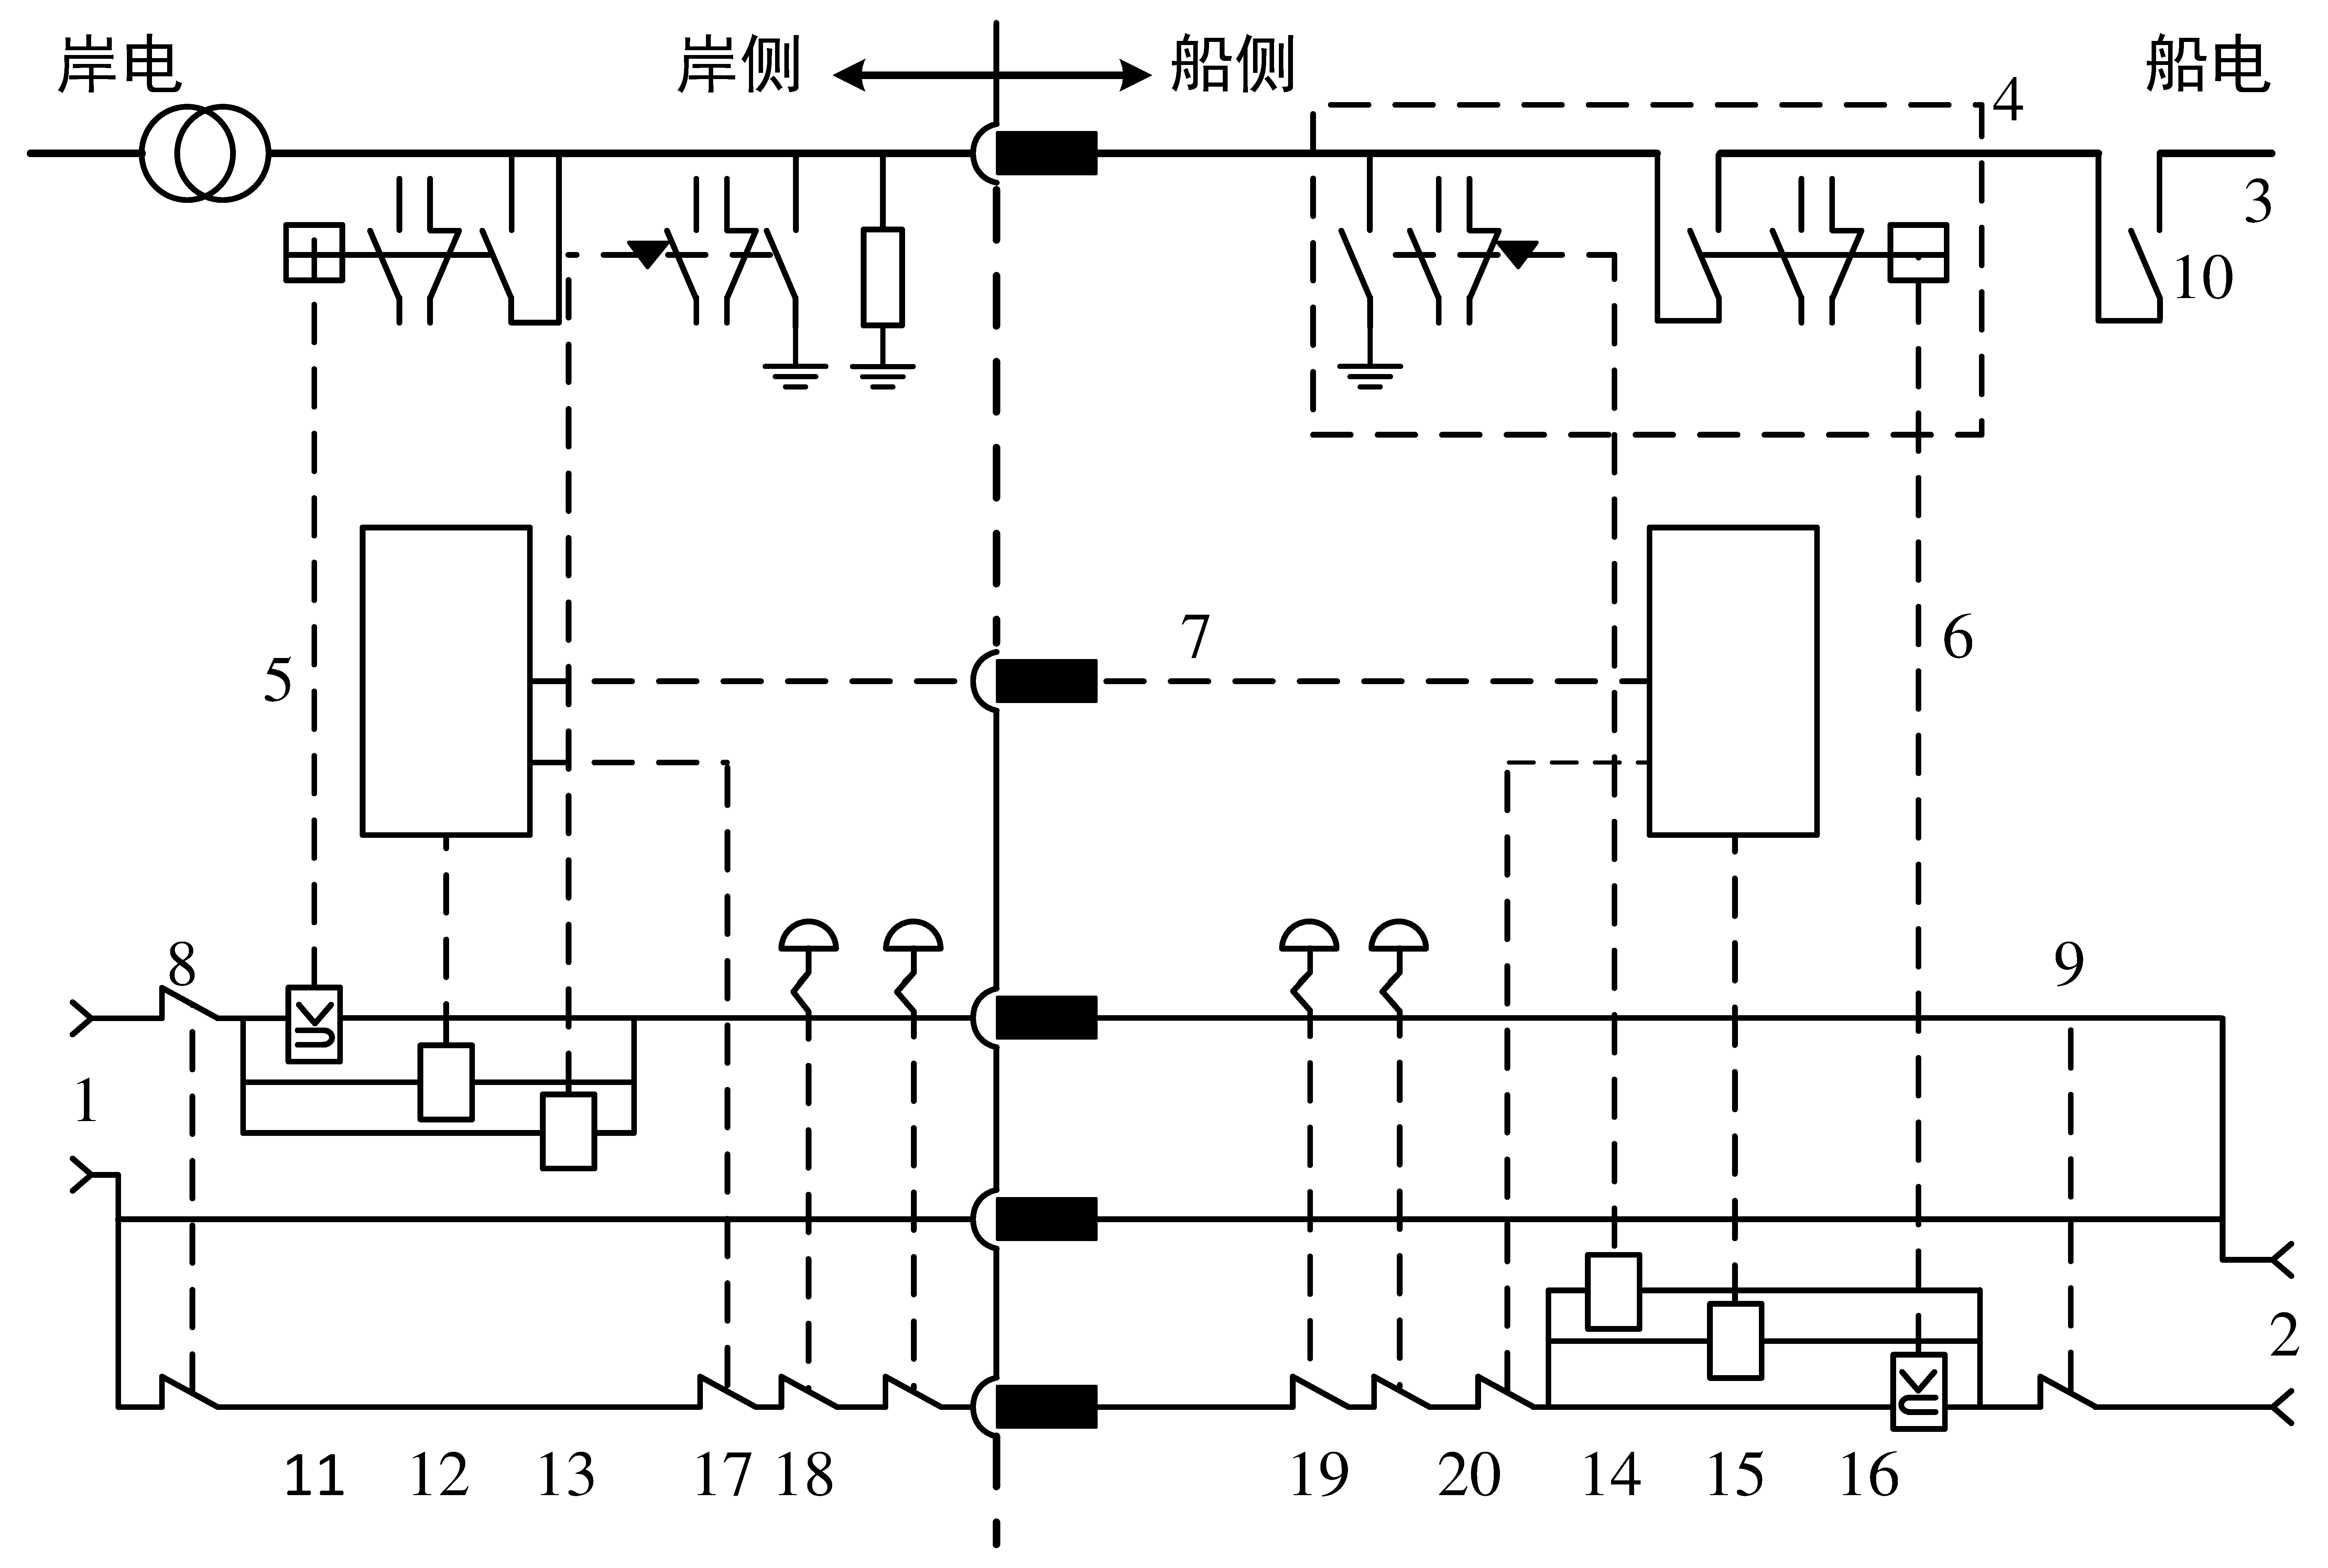
\includegraphics[width=0.8\textwidth]{chapter5/岸电电源控制系统原理图.pdf}
	\caption{岸电电源控制系统原理图}
	\label{fig:岸电电源控制系统原理图}
    {\kaishu \zihao{5}
    \hspace*{\fill} 

    1-岸侧控制电源;2-船侧控制电源;3-船舶电网;4-船电岸电切换柜;

    5-岸电PLC控制器;6-船侧PLC控制器;7-光纤通信;8-岸电保护;

    9-船电保护;10-同步切换开关;11-岸电切换开关;12-岸电保护开关;
    
    13-岸侧接地允许;14-船侧接地允许;15-船侧安全保护;16-船侧切断开关;

    17-船侧接地控制;18-船侧手动接地;19-岸侧控制接地;20-岸侧手动接地;

    }
\end{figure}

\section{第一节}

\subsection{子节点}